\section{Magneto-Inertial Fusion with Magnetic Mirrors - Environmental Analysis}

\subsection{Introduction}

The matter of the environmental impact of fusion is, for many, a key motivating factor for its development. In this review, an overview of the relevant literature is presented. These broadly focus on the direct environmental impacts of fusion power plants (section \ref{sec:direct_imp}) and a more macroscopic view of the impact of widespread fusion adoption on the environment and climate change, and the interdependent role of policy. Following this, a focus is given to the extraction and processing of lithium, as one of the most important, but potentially most limited and environmentally impactful resources required for fusion. Finally, the relevant considerations discussed in the literature review are applied to the specific case of the MIF concept presented in this report. Issues including tritium management, comparative environmental impact, land requirements, and economic viability within the context of environmental policy frameworks are discussed.

\subsection{Literature Review}

\subsubsection{Fusion Power Plant Direct Environmental Impacts}

\label{sec:direct_imp}
In 'Nuclear Fusion Power and the Environment', 1974, Hirsch and Rice survey the practical feasibility and environmental impact of fusion energy \cite{hirsch1974nuclear}. They consider Tokamak, theta pinch, mirror and and laser-driven approaches. The paper addresses the following environmental concerns:
\begin{itemize}
    \item Tritium waste: a reference power plant reported a tritium leakage of 0.0001\%, based on a system with a 6kg reserve. The maximum dosage this level of leakage could give is 1 mrem/year, or 1\% of the average dose to the population from background sources. Tritium is described as 'well-characterized isotope and one of the less hazardous radioactive nuclides', but says that more research into tritium safety is needed.
    \item Land requirements: fusion power plants 'should require no more land than present-day fission power-plants, and the fusion fuel storage requirements will be negligible'.
    \item Fuels and Materials supply: 'The fuel deuterium is obtained from water and is
essentially an infinite fuel resource', and it's use results in the production of useful quantities of hydrogen and oxygen. The study describes the supply of terrestrial lithium as being sufficient for '2,900 years of energy demand' for tritium production, and does not foresee the exponential increase in demand for use in batteries. It goes on to highlight seawater as a limitless supply of lithium, but does not elaborate on the environmental impact of its extraction.
\item Ore requirements: copper and lead are highlighted as demanding the greatest ore usage. The study expresses concern over a worldwide shortage of these metals.
\end{itemize}

In 'The environmental impact of fusion power', 1989, Atkinson focuses heavily on the tritium fuel cycle and the radiation challenges is could present \cite{atkinson1989environmental}. Atkinson highlights the similarity tritium has with hydrogen, thus its propensity to diffuse through solid materials, meaning 'rounding atmosphere will therefore constantly need purging'. It can also form tritiated water, which is more hazardous, but easier to handle. Atkinson continues to describe how structural materials could become activated, becoming radioactive waste themselves 'the fusion reactor vessel itself becomes a heavily  radioactive object with a complex profile of radiation products'. It is stated that this issue could be addressed by careful selection of low-activation structural materials. Atkinson describes contemporary environmental studies such as ESECOM as 'consistently optimistic when compared with the US literature'. The study concludes with 'if the solutions  currently hoped to be achievable in the fusion field  are, in practice, achieved then this will result in a far less hazardous energy source than any of the fission options'.
\\\\
In 'Environmental aspects of fusion energy', 1991, Rytov identifies anthropogenic changes in the atmosphere to be a matter of high concern, and that only fission, fusion and possibly solar can meet the baseload requirement as an alternative to fossil fuels \cite{rytov1992environmental}. Rytov identifies and addresses the following assessment criteria to evaluate environmental impact of an energy technology: 
\begin{itemize}
    \item Resources of fuel. Deuterium: abundant and easily obtained from water (does not minimize the environmental impact of extraction). Lithium: $^6$ Li is required, but only 300kg is needed for a 1GW system.
    \item Resources of other materials. Rytov claims that fusion reactors do not depend exclusively on any single construction material. One challenge is the acquisition of helium as a coolant, and additional investment in helium production will be needed to meet demand.
    \item Land requirements. Land requirements are similar with those of coal or fission power plants, and two orders of magnitude less than solar.
    \item Radioactive Hazards . The fusion reaction cannot self-accelerate and self-quenches. Also, only $\sim$ 200 mg of Tritium is available to react, corresponding to around ten seconds of operation, making a Chernobyl-like disaster theoretically impossible. The most dangerous source of Tritium is identified as being contained in the blanket. In the scenario that the entire inventory was released, there would be no fatalities due to acute radiation syndrome beyond 1km.
    \item Waste disposal. The construction materials required are of similar magnitude to a fission power plant, so industrial waste during construction is 'not a matter of concern.' The radioactive waste is 'approximately 100 times less radioactive than for a fission reactor'. Use of low-activation structural materials would reduce this further.
\end{itemize}

In 'Is nuclear fusion a sustainable energy form?', 2011, Bradshaw et al. defines a sustainable energy source in the consumption of natural resources as one with an effectively limitless supply, correlating to a few million years \cite{bradshaw2011nuclear}. The paper finds that lithium and deuterium satisfy this criteria, due to their abundance in seawater. However, it is likely that all terrestrial sources of lithium will be exhausted for use in batteries over the next few decades, meaning a sustainable means for extraction of lithium from water is needed. The paper identified helium as another resource that could represent challenges.

In 'Fusion power in a future low carbon global electricity system', 2016, Cabal et al. used a model of the worldwide energy system (called TIMES) to observe the effect varying implementations of fusion power on a future low carbon global electricity system \cite{cabal2017fusion}. Three scenarios were analyzed, varying in global prioritization of decarbonization. The paper concludes that the scenario with the strongest environmental responsibility will see the greatest implementation of fusion reactors. Furthermore, the discount rate is a significant factor, with lower rates resulting in greater penetration of fusion, and CCS technologies being favoured by a higher discount rate.

In 'Summary of the 1st International Workshop on Environmental, Safety and Economic Aspects of Fusion Power' 2016, presentations focused on potential safety and local environmental issues presented by tritium \cite{wu2016summary}. Notable points include that ITER serves as an important learning point for the industry, both in terms of safety policy and implementation. A description of the possible hazards presented by tritium embedded in tungsten dust was given; a particular risk occurs when the dust is at low temperature (100 °C) in contact with the tritium gas. Tritium release is slower if tungsten dust is in aqueous solution and faster under acidic conditions. It was emphasized that socioeconomic considerations are essential and should be reflected in the plant design to maximize the possibility of the adoption of fusion power for future energy markets. It was stated that fusion must "have the capability to produce alternative fuel particularly bio-based, and have significant relevance to CO2 emission reduction". It was stated that 'fusion has a chance to succeed only under strong environmental constraints', such as in the SRES A1T scenario in which the global population peaks in the middle of the twenty-first century with rapid economic growth and CO2 emission reduction.

In 'Potential of Nuclear Fusion Energy Source for a Sustainable Future', 2021, Christy and Tammisetti analyze a scenario for a new fusion company with the aim of achieving commercial fusion \cite{christy2021potential}. The model incorporates various techno-economic factors. The first step of the analysis evaluated 'if nuclear fusion energy source is the future'. This involved consideration of environmental factors, including resource sustainability, CO$_2$ emissions, and radioactive waste. The analysis found that fusion fuels are widely available, with deuterium and lithium being extractable from water, (300 l provides approximately 1g of deuterium) and tritium being produced in the reaction of neutrons with lithium. The scenario determined minimal production of CO$_2$ and other greenhouse gases, with the major by-product being helium. Finally the scenario stated that radioactive waste could be re-used after 100 years, provided low activation materials were used.


\subsubsection{Effect of Global Fusion Implementation and Policy on the Envrionment}
\label{sec:pol}

In 'Role of nuclear fusion in future energy systems and the environment under future uncertainties', 2003, Tokimatsu et al. study the time frame by which fusion could become competitive in the energy market, under various policy schemes and economic conditions \cite{tokimatsu2003role}. The investigation found that the economic viability of fusion is dependent on targets for CO$_2$ concentration, discount rate and design, in the scenario that present-day Tokamak designs are constructed, with a CO$_2$ concentration constraint  of 550 ppmv, fusion could see competitive implementation in 2050-60.  The report highlights the benefits of widespread fusion adoption as reduced energy cost and mitigated carbon tax.
The Appendices for this study include a discussion of the resources required for fusion and address each as follows:
\begin{itemize}
    \item Deuterium: presently, plants in Canada are capable of providing 800 tonnes of D$_2$ per year, which is approximately 11 000 times the requirement of a 1 GW DT fusion power plant. Little energy is consumed in the process, as the process is based on equilibrium chemical reactions.
    \item Tritium: assuming 304 tonnes of tritium to be consumed during 30 lifetime of a 1 GW Tokamak, it was found that to supply half the world's energy (1500 1 GW Tokamak fusion reactors), 15 kTons of lithium would be required annually. This correlates to 600 years in the reserve base, or 1.5 million years when considering that available from seawater.
    \item Beryllium: the global mineral reserve of Beryllium is estimated to be 100 MTons, and to construct and maintain 1500 1 GW reactors, 165 kTons are required annually. This implies a resource lifetime of 430 years from the reserve base, or 70 000 years to consume the mineral supply.
\end{itemize}

In 'Clean and Sustainable Fusion Energy for the Future', 2014, Adelerhof et al. discuss the various MCF approaches to fusion, and compared with other energy sources including solar, wind and coal \cite{adelerhof2014clean}. A large part of this comparison is environmental. The study notes that 88\% (as of 2014) of global energy is supplied by fossil fuels and that these will likely be exhausted by the end of the century (see table \ref{tab:resource_supply}). Adelerhof et al. find that an alternative to fossil fuels is urgently needed, and that whilst fusion could be an important part of this, it is not likely to be commercially viable until 2050, so other need to be implemented in the short term. The paper concludes with the statement 'fusion power should be adopted worldwide and if done so will provide the world with limitless clean energy billions of years into the future'. 

\begin{table}[h!]
    \centering
    \begin{tabular}{lcc}
    \hline
       \textbf{Fuel}  & \textbf{Proved Recoverable Reserves} & \textbf{Years of Use at Current Rate of Consumption}\\
       \hline
      Coal  &$1 \times 10^{12}$ tons & 270  \\
      Crude Oil & $9.5 \times 10^{11}$ barrels & 40-50  \\
      Natural Gas & $1.2 \times 10^{14}$ m$^3$  & 60-70  \\
      Uranium & $2 \times 10^{6}$ tons  & 40-50 (2400-3000)*  \\
      \hline
    \end{tabular}
    \caption{The number of years worth of energy supply remaining for the four most dominant forms 
of energy supply for the world (as of 2004), adapted from \cite{adelerhof2014clean}. *If breeder technology is employed.}
    \label{tab:resource_supply}
\end{table}

In 'Nuclear energy and sustainability: Understanding ITER', 2006, Fiore sets out three requirements for ITER (or fusion reactors in general) to be sustainable: availability ('provide energy with a low consumption price and easily accessible infrastructures and technological know-how'), accessibility (fusion power should be as abundant and cheap as possible) and acceptability (fusion power must be ecologically safe to be accepted) \cite{fiore2006nuclear}. Fiore concludes that fusion power must be coupled with other renewable energies, particularly in the short term, and particularly in the global south.

In 'Approximation of the economy of fusion energy', 2018, Entler et al. discusses the economics of fusion energy, with discussion of environmental factors from an economics perspective \cite{entler2018approximation}. They state that 'the environmental impact of fusion power plants will be comparable to the impact of renewable resources'. A breakdown is provided of the ExternE evaluation of
external costs of energy. Three main impacts are identified damage to human health
(increased risk of mortality and morbidity), effects on ecosystems
and biodiversity (changes in the environment, biodiversity loss)
and the impact on resources and depletion (mainly of water, metals
and fuels, but also crops, buildings, etc.). The results for fusion in comparison with other energy solutions are provided in \ref{fig:externE}

\begin{figure}[h!]
    \centering
    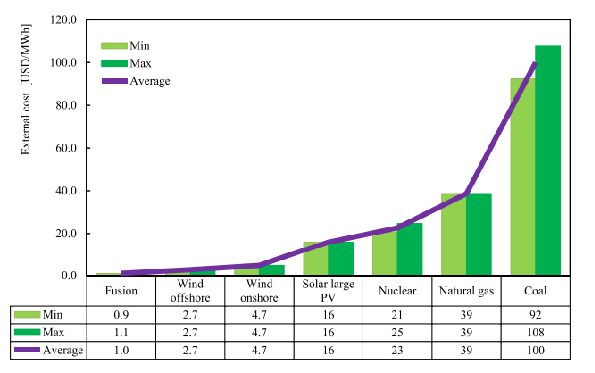
\includegraphics[width =0.65\linewidth]{SubreportFigures/externE_comp.pdf}
    \caption{ External costs of selected energy sources according to the ExternE methodology from \cite{entler2018approximation}.}
    \label{fig:externE}
\end{figure}

In 'Socioeconomic and environmental impacts of bringing the sun to earth: A
sustainability analysis of a fusion power plant deployment', 2020, Banacloche et al. an overview is given of the environmental impacts of fusion, along with economic and social factors \cite{banacloche2020socioeconomic}. The environmental cost is described as 'in the same range as the external costs of photovoltaics and wind energy'. Furthermore, a breakdown of the CO$_2$ emissions is given for each sector within the fusion supply chain. It identifies mining and quarrying in the USA and manufacture of basic metals as the biggest contributors, with total CO$_2$ emissions of 755 and 675 kT for the lifetime of the plant.

In 'Potential contribution of fusion power generation to low-carbon development under the Paris Agreement and associated uncertainties', 2020, Gi et al. assess the potential contribution of fusion energy towards the 2\degree C 2100 target as set out by the Paris agreement \cite{gi2020potential}. Canada and Japan mentioned fusion as a possible tool in this target in their 2019 long-term strategies. The probability of meeting this target, uncertainties in development, and outlook for commercialization are evaluated using a global energy model (DNE21$+$) under various scenarios. The conservative R\&D in fusion model found Japan, Korea and Turkey to be the most commercially competitive regions for fusion, due to lack of viability of zero-emission alternatives. Beyond this, the study finds that 'If inexpensive power plants could be developed by enhanced R\&D and advanced design in DEMO projects, fusion power plants will also contribute to decarbonization in the EU28, India and China. A full comparison of required fusion energy cost under various scenarios can be seen in \ref{fig:breakeven}. Increasing path number corresponds to increased aggression of CO$_2$ target, increased SSP number corresponds to decreasing global action. See \cite{gi2020potential} for details of scenarios.

Further cost reduction, by innovative design and alternative concept, will become essential for fusion plants to contribute to decarbonization in zero-emission resource-rich countries.'. Finally, Cabal et al. emphasize the importance of funding fusion energy, so that it can play a role in meeting the 2\degree 2100 target.


\begin{figure}[h!]
    \centering
    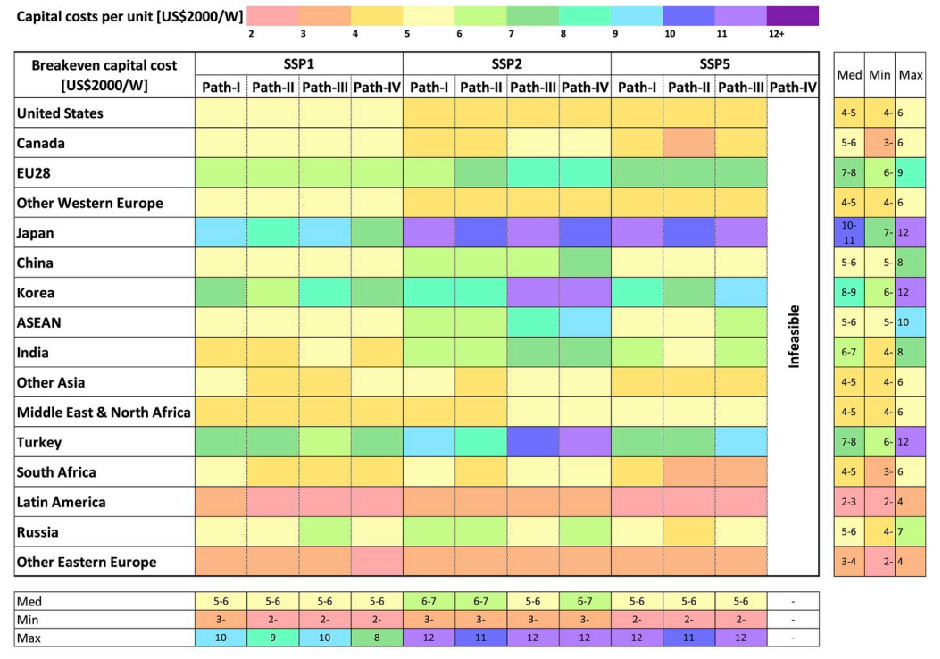
\includegraphics[width =0.65\linewidth]{SubreportFigures/breakeven_by_nation_co2.pdf}
    \caption{ The required breakeven price of a fusion reactor per Watt generated, for various regions. The groups SSP1, SSP2, SSP3 correspond to decreasing global action on climate change, and the four paths correspond to various CO$_2$ concentration changes as follows: temperature overshoots 2\degree C increase before 2100 but declines to below 2\degree C by 2100; stabilization below 2\degree C under climate sensitivity of 2.5\degree C;  stabilization below 2\degree C under climate sensitivity of 3\degree C; stabilization at 450-ppmv CO$_2$ by 2100. Adapted from \cite{gi2020potential}. }
    \label{fig:breakeven}
\end{figure}

In 'Nuclear energy consumption, nuclear fusion reactors and environmental quality: The case of G7 countries', 2022, Cakar et al. investigate 'the impact of nuclear energy consumption and technological innovation on environmental quality in G7 countries', including an analysis on the impact of nuclear fusion \cite{ccakar2022nuclear}. Cakar et al conclude that 'Researches on nuclear fusion reactors need to be encouraged to contribute to reducing the environmental costs of nuclear
energy', and that the main benefit of fusion in comparison to fission, is that it produces more energy with less fuel and that 'this advantage brings a reduction in environmental degradation'. Additionally, technological advancement in fusion energy improves the negative public perception of nuclear energy in G7 countries.

\subsubsection{Environmental Impact of Lithium Extraction and Processing}
%Lithium

As the primary source of tritium both in this concept, and in most fusion concepts with tritium fuel, the environmental impact of lithium extraction and processing is a key issue. Although the quantity of lithium required for a single fusion reactor may be relatively low (300 kg according to one estimate \cite{rytov1992environmental}), this will vary between concepts, blanket designs, and the efficiency of tritium recovery, and if fusion power is to be a globally significant energy source, the matter of its extraction is vital. 

This section presents key environmental concerns associated with lithium, and the outlook for fusion. It should be noted that presently, the topic of the environmental impact of lithium is grossly under-researched. As a key resource not just for fusion, but for the exponentially growing battery industry, the sustainability of it's extraction and life-cycle could become a key environmental issue over the course of the century. 

In 'Environmental impact of direct lithium extraction from brines', Vera et al describe the two currently implemented means of lithium extraction: mining hard rock ores and evaporation of continental brine \cite{vera2023environmental}. Both supplies are limited and have significant disadvantages including the slow extraction rate, low sensitivity to changes in demand, significant environmental impact (in terms of local damage, extremely high water usage, and carbon footprint), and the fact that both supplies are extremely geographically localized; 85\% lithium extraction is in the 'lithium triangle' in South America, with much of the rest in China. A third option is the broad field of 'direct lithium extraction' (DLE)'. The focus of the paper is to compare the environmental impact of these upcoming technologies. Various DLE approaches are identified: ionic exchange resins, organic solvents or solutions, membrane processes, electrochemical ion-pumping technology, selective precipitation and concentration of native brines with concomitant water recovery. Vera et al. considered each through the lenses of freshwater usage, energy demand, and scaling requirements and potential. Ion pumping and Li$^+$-selective membranes are identified as promising but immature technologies that need 'ample engineering efforts to reach industrial scale'. Solvent extraction, and some electromembrane and thermally assisted brine concentration processes,  'large-scale plants for the separation of other chemicals are already in place and equipment could be adapted fairly easily'.

\begin{figure}[h!]
    \centering
    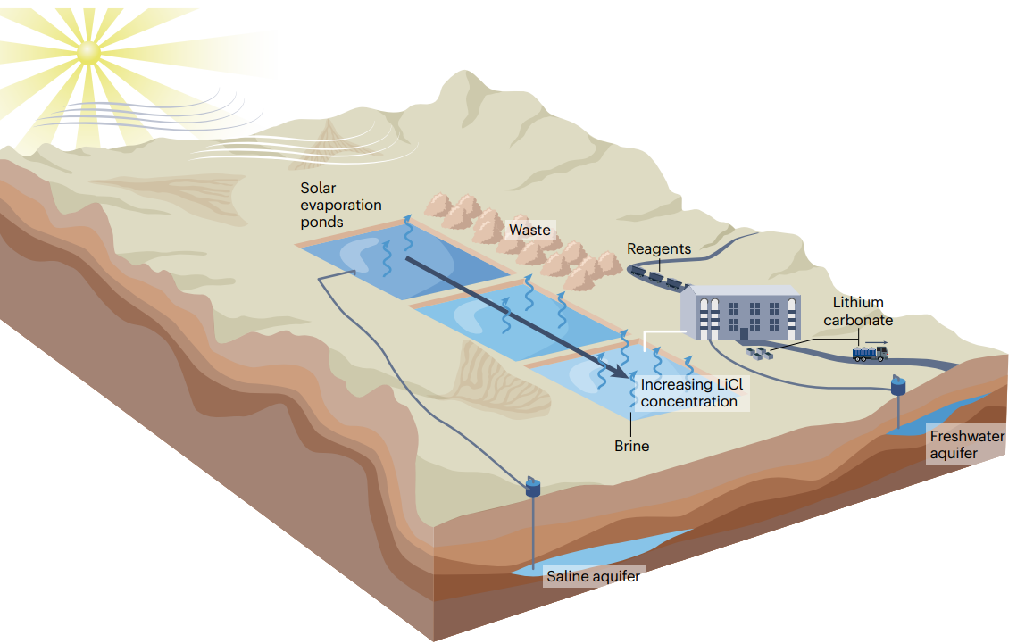
\includegraphics[width =0.65\linewidth]{SubreportFigures/brine_lake.pdf}
    \caption{Schematic diagram of typical brine lake lithium extraction.  LiCl concentration 
increases gradually and salts from other cations crystallize in the ponds as 
saturation is reached. Concentrated brines then enter a refining plant for 
crystallization of the final product (usually lithium carbonate). Fresh water and 
chemicals are used at several steps of processing. From \cite{vera2023environmental}. }
    \label{fig:circ_economy}
\end{figure}

It was identified that for each tonne of Li$_2$CO$_3$, 115 tonnes of waste were produced. The study advocates a 'circular economy approach' in which other resources including magnesium, potassium, calcium, sodium, fresh water, and boron products could be extracted (see \ref{fig:circ_economy}). The study called for more research on the water usage of various DLEs, the local environmental impact of both existing evaporative brine extraction and upcoming DLEs, and for sustained environmental observation before, during, and after lithium extraction at a location.

\begin{figure}[h!]
    \centering
    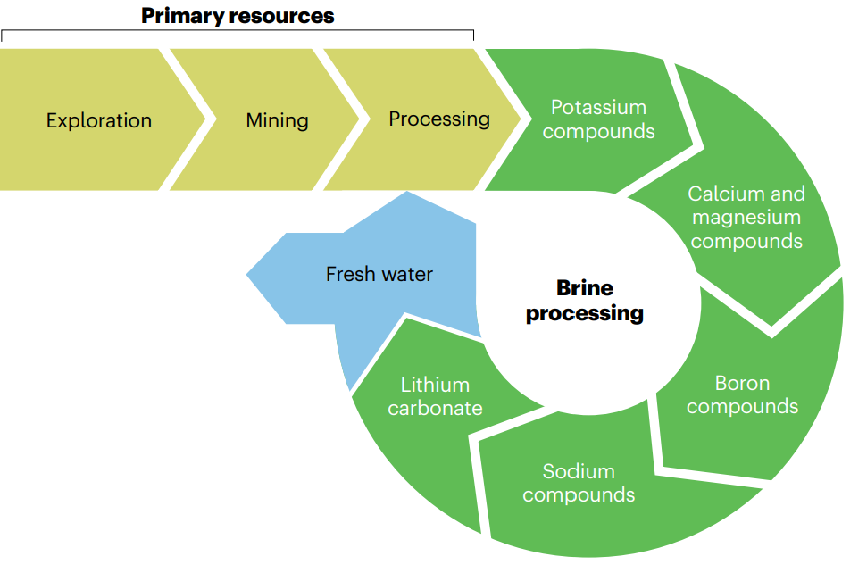
\includegraphics[width =0.65\linewidth]{SubreportFigures/circ_economy.pdf}
    \caption{Proposed 'circular economy' approach where other resources besides lithium are extracted. From \cite{vera2023environmental}. }
    \label{fig:circ_economy}
\end{figure}

In 'Socio-environmental impacts of lithium mineral extraction: towards a research agenda', Buyung Agusdinata et al. offer a meta-analysis focusing on socio-economic and environmental studies relating to lithium extraction between 1974 and 2020 \cite{agusdinata2018socio}. The study notes that most environmental assessments focus on the impact of end-of-life lithium-ion batteries used for electric vehicles. In this case, greenhouse gas emissions are dominated by the manufacturing process, not by the lithium extraction itself ($\sim$ 110 g CO$_2$ per Watt hour of battery storage). The largest environmental concern in the extraction is the use of evaporation ponds - 'Since geochemically lithium is a highly mobile element, there is a high chance that lithium will be released into the environment and potentially affect nearby communities'. There is also a risk of local water contamination due to a failure in the PVC liners of the evaporation ponds. The risks for human health and native biodiversity may be severe, but are currently poorly understood.

In 'Environmental impacts of a transition toward e-mobility: the present and future role of lithium carbonate production', Stamp et al. conduct a life cycle assessment on the production of Li$_2$CO$_3$ from natural brines, ores and seawater \cite{stamp2012environmental}. The study found that the CO$_2$ emmission from lithium extracted from brine or ore is comparable, with a carbon footprint of 2.02 and 2.27 kg CO$_2$-eq per kg of Li$_2$CO$_3$ extracted, respectively. Extraction from seawater, however, has $\sim$7000\% the carbon emission per kg of lithium produced, compared with the two conventional processes. The total stock of lithium in seawater is $\sim$2.4$\times 10^{11}$ tonnes, although the concentration is only 0.173 ppm - ten thousand times less than the currently exploited brines. This means that vast amounts of seawater would need to be processed, about 5430 m$^3$ for each kilogram of lithium extracted. It is noted, however, that there is currently no quantitative data relating to the extraction of lithium from seawater, as it has still yet to be done. The requirement for extraction of lithium from seawater is dependent on the innovation in DLEs for brine lakes, and the efficiency of end-of-life recycling. The paper concludes that the greenhouse gas emissions of lithium extraction are negligible (in battery production) until (or if) extraction from seawater becomes the main source.


\subsection{Environmental Impact of Magnetic Mirror Fusion}

There have, as of writing this report, been no published studies on the environmental concerns specific to a MIF power plant. In this section, relevant literature is applied to the specific design features of the MIF presented in this report. Key features include the use of DT fuel, the PbLi blanket, the large magnetic coils and the accompanying cryogenic systems, and how MIF may be specifically impacted by, or respond to policy.

\subsubsection{Tritium Management in MIF with Mirrors}

The MIF desiogn presented here utilizes DT fuel. Although tritium is 'one of the less hazardous radioactive nuclides', it still represents the potential for significant ecological damage, thus the issue of containment and handling must be prioritised \cite{hirsch1974nuclear}. Atkinson's 1989 study highlights tritium's ability to diffuse through solid materials, requiring continuous purging of the atmosphere. The possible production of tritiated water, adds complexity to these challenges, and should be considered carefully in the design \cite{atkinson1989environmental}.

Moreover, the MIF with mirrors concept must address radiation challenges related to structural materials. Tritium and other radioactive materials can irradiate the reactor vessel, primary structure, shield , blanket, and any tritium-facing sensors and instrumentation. Development and implementation low-activation materials for the reactor’s structure, including magnetic coils and PbLi blanket, is a 'critical path to fusion power' \cite{moslang2005towards}. 

\subsubsection{Comparative Environmental Impact}
The environmental impact of fusion power plants, including the MIF with mirrors design, is expected to be comparable to that of renewable resources. Banacloche et al.'s 2020 analysis of the environmental impacts of fusion power suggests that the environmental costs are in the same range as those of photovoltaics and wind energy \cite{banacloche2020socioeconomic}. This comparison is important for the MIF with mirrors concept as it positions fusion as a viable alternative to other renewable energy sources, particularly in terms of its effects on human health, ecosystems, and resource depletion. Furthermore, as a pulsed confinement concept (as opposed to a steady-state configuration such as a Tokamak), the MIF reactor is a dispatchable power source, and can prioritise power output in times of low renewable power generation. This potential for synergism opens up markets for implementation (such as those with high solar penetration), and will contribute to a greater zero-carbon share of the energy sector.

\subsubsection{Land Requirements}
The MIF power plant design presented here should have a comparable site size to that of existing plants, offering an advantage when compared to, for example hydroelectric or solar, which can have a marked impact on local ecology \cite{fletcher2010environmental}.

\subsubsection{Economic Viability and Policy Frameworks}

A key finding of this part of the report is that the viability and implementation of fusion energy is closely linked to environmental policies and economic conditions. The MIF concept presented in this report is no exception. The study on this matter performed by Tokimatsu et al. found that fusion could become competitive in the energy market under various policy schemes, particularly those targeting CO$_2$ concentration and discount rates \cite{tokimatsu2003role}. For instance, if modern Tokamak designs are constructed with a CO2 concentration constraint of 550 ppmv, fusion could see competitive implementation between 2050 and 2060. Although MCF approaches have been the mainstream research in fusion for the last three decades, and have enjoyed orders of magnitude more funding than MIF,  they have yet to demonstrate $Q > 1$. MIF has exhibited an extremely high rate of growth in the last decade, and could challenge MCF to be the first commercially viable fusion concept. As such, it would be beneficial to perform a similar analysis on MIF concepts to that performed by Tokimatsu et al. on Tokamaks.
